\section{Experiments}\label{sec:experiments}

\subsection{Certified Test-set Accuracy}\label{subsec:certified-test-set-accuracy}
In the context of adversarially robust classification, the concept of certified radius plays a crucial role.
However, it is important to note that the certified radius is calculated only at a given point.
This localized measure, while useful, does not provide a comprehensive understanding of a classifier's robustness across the entire input space.
To address this limitation, practitioners use a global measure for smoothed classifiers obtained through randomized smoothing, called the \textit{certified test-set accuracy} (CTA).

Let $g$ be a classifier, $S = \{(x_1, c_1), \ldots, (x_N, c_N)\}$ be a test set, and $r$ be a radius.
We define an indicator function for each example $i \in [N]$:

\[
    z_i(r) = \mathbbm{1}[g(x_i + \delta) = c_i \quad \forall \|\delta\|_2 < r]
\]

The theoretical certified test-set accuracy at radius $r$ is then defined as:

\[
    \text{CertAcc}_{\text{theo}}(r) = \frac{1}{N} \sum_{i=1}^N z_i(r)
\]

This measure represents the fraction of the test set that $g$ classifies correctly with predictions that are certifiably robust within an $\ell_2$ ball of radius $r$.

For randomized smoothing classifiers, computing the theoretical certified test-set accuracy exactly is not feasible.
Instead, we introduce the \textit{approximate certified test-set accuracy}.

Let $Y_i(r)$ be a Bernoulli random variable denoting the event that, for example $i$, estimating the certified radius of the smoothed classifier returns a certified radius $R$ which is greater than $r$.
The approximate certified test-set accuracy is then:


\[
    \text{CertAcc}_{\text{approx}}(r) = \frac{1}{N} \sum_{i=1}^N Y_i(r)
\]

Importantly, $Y_i(r) = 1$ does not necessarily imply $z_{i}(r) = 1$.
However, if $z_i(r) = 0$, then $P(Y_i(r) = 1) \leq \alpha$.
This relationship allows us to construct a one-sided confidence interval for the unobserved quantity $\frac{1}{N} \sum_{i=1}^N z_{i}(r)$ using the observed quantity $\sum_{i=1}^N Y_i(r)$ (see Theorem 6 in~\citep{cohen2019certified}).

\subsection{Results}\label{subsec:results}

To compare our new radius estimation methods with the standard approaches, we run our experiments on the CIFAR-10 dataset.
Results for the Imagenet dataset can be found in Appendix~\ref{sec:more-experimental-results}.
The failure rate $\alpha$ is chosen to be $0.001$ throughout all the experiments.
The base classifier $F$ is the same 110-layer residual network from~\citep{cohen2019certified}, trained using Gaussian noise data augmentation, such that the standard deviation $\sigma$ of the Gaussian noise used during training is the same one used when smoothing the base classifier.

In all the figures, the CTA curves that are plotted are actually based on the margins instead of the radii since they are directly proportional (meaning we only estimated margins instead of radii), hence we use them interchangeably in our analysis.
To explain how to read one of our figures, we can take for example Figure~\ref{fig:discrete_sigma}.
We have six comparisons, in the first three comparisons (on top), the certified radius that was chosen is the first radius (Equation~\eqref{eq:first-radius}), and it was estimated for all examples of the test set in order to obtain the CTA curve (same thing goes for the second radius on the bottom).
As explained in this Section~\ref{subsec:practical-calculation-of-confidence-interval}, we can estimate the certified radius using the Bonferroni correction alongside an exact one-sided confidence interval (as outlined in Algorithm~\ref{alg:bonferroni}).
The Bonferroni approach is agnostic to the type of confidence interval being used, which leaves us with the choice of the confidence interval that is indicated in the legend of the plot after a plus sign.
The `Ours' keyword in the legend indicates that the radius was estimated using the methods that we have explained in Section~\ref{sec:discrete} and Section~\ref{sec:continuous}.
In the continuous case, we have just outlined a high-level approach without specifying which confidence interval to use, which means that our approach (like the Bonferroni approach) is agnostic to the choice of confidence interval.
In this paper, we mentioned two methods to obtain confidence intervals for the mean of a continuous random variable: the empirical Bernstein inequality (Proposition~\ref{prop:empirical-bernstein-inequality}) which we refer to in the legends as `Bernstein' and the betting confidence sequence (Proposition~\ref{prop:confidence-sequence}) which we refer to in the legends as `CS'.
This leaves us with a maximum of $2\times2$ possibles combinations.

Starting with the discrete case, there are two main hyperparameters that influence the shape of the CTA curve: the number of samples $n$ and the standard deviation $\sigma$.
The easiest hyperparameter dependence to analyse is the number of samples $n$.
As Figure~\ref{fig:discrete_num} and Table~\ref{tab:simplified-certified-accuracy} show, the standard Bonferroni approach is far more conservative when the number of samples is small, although as the sample size increases, the impact of this correction becomes less significant, and the two curves end up converging and overlapping as a natural consequence of improved statistical estimation, reduced conservatism in bounds, and diminished impact of discretization effects.
It is also worth noting that the second margin takes much more samples to converge than the first one which is linear, and the differences are much more pronounced at larger radii.

\begin{figure}[htbp]
    \centering
    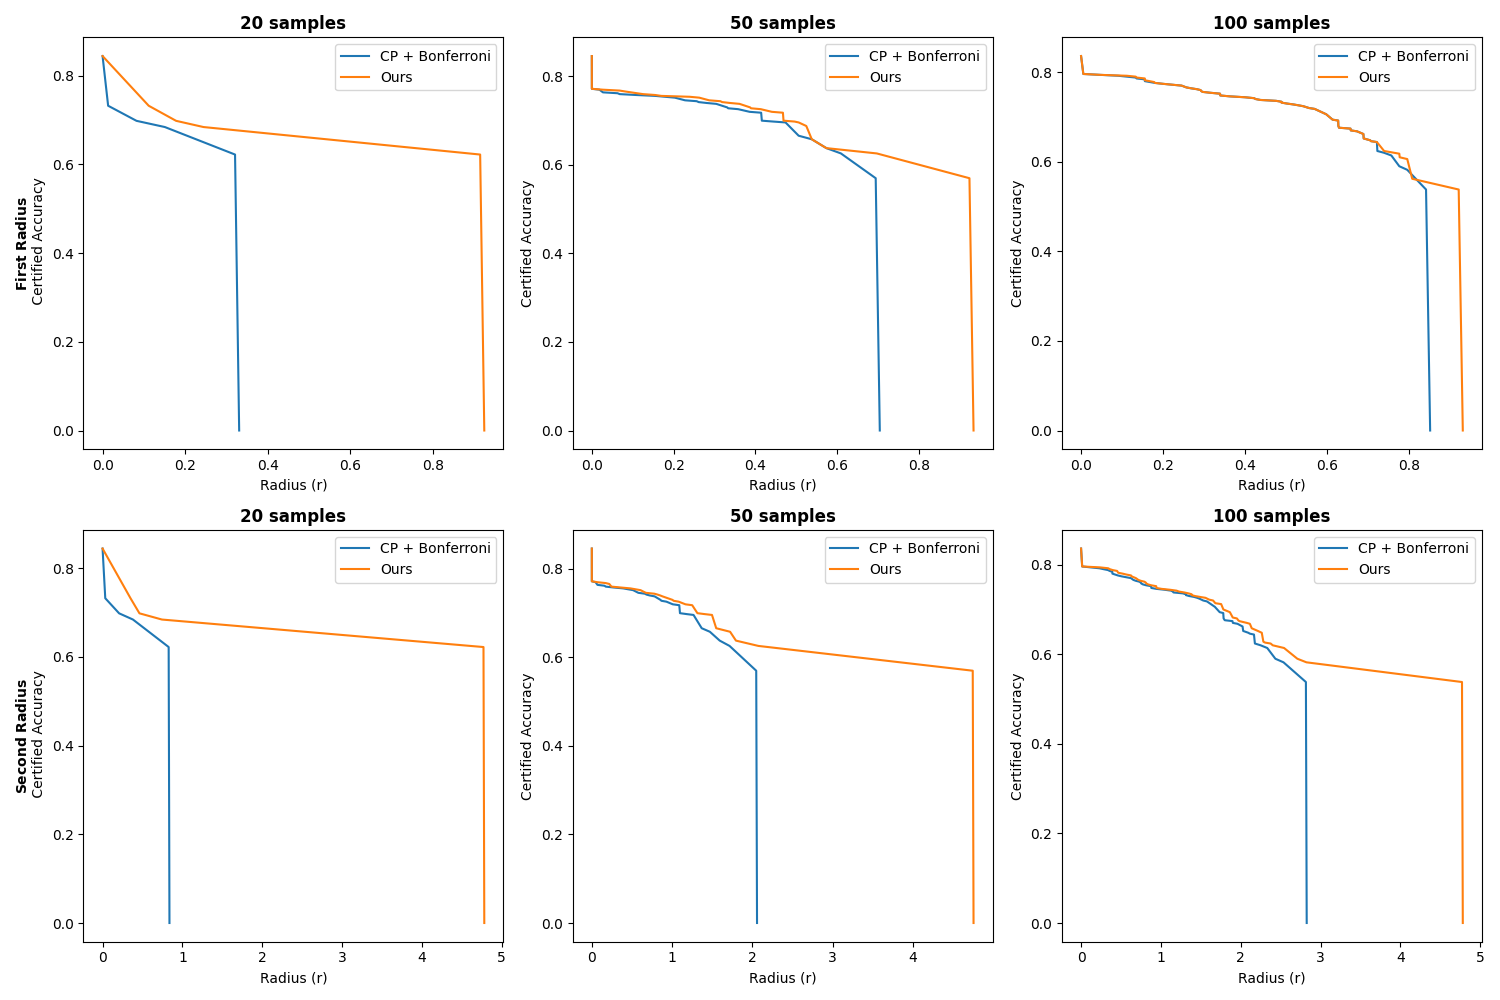
\includegraphics[width=0.8\textwidth]{images/discrete_num}
    \caption{Certified accuracies' comparison on the CIFAR-10 dataset in the discrete case for different numbers of samples (displayed on the columns) with $\sigma = 0.12$. CP + Bonferroni means Clopper-Pearson interval with Bonferroni correction, and Ours means our new approach in section~\ref{sec:discrete}. The first row compares the certified accuracies using the first margin and the second row compares the certified accuracies using the second margin.}
    \label{fig:discrete_num}
\end{figure}

\begin{table}[htbp]
    \centering
    \caption{Certified accuracy using the second margin on the CIFAR-10 dataset in the discrete case for different values of radius $r$ with a sample size of $100$ and a standard deviation $\sigma = 0.12$.}
    \label{tab:simplified-certified-accuracy}
    \renewcommand{\arraystretch}{1.2}
    \begin{tabular}{l*{9}{c}}
        \toprule
        Method & \multicolumn{9}{c}{Radius ($r$)} \\
        \cmidrule(l){2-10}
        & 0.5 & 1.0 & 1.5 & 2.0 & 2.5 & 3.0 & 3.5 & 4.0 & 4.5 \\
        \midrule
        CP + Bonferroni & 0.774 & 0.744 & 0.720 & 0.662 & 0.582 & 0.000 & 0.000 & 0.000 & 0.000 \\
        Ours              & 0.780 & 0.746 & 0.726 & 0.670 & 0.614 & 0.538 & 0.538 & 0.538 & 0.538 \\
        Gain (\%) & 0.78\% & 0.27\% & 0.83\% & 1.21\% & 5.50\% & $\infty$ & $\infty$ & $\infty$ & $\infty$ \\
        \bottomrule
    \end{tabular}
\end{table}

The second most important hyperparameter to consider is the standard deviation $\sigma$.
As Figure~\ref{fig:discrete_sigma} shows, when the standard deviation increases, the CTA decreases as the classifier’s base accuracy decreases because the added noise makes the classification task harder, leading the model to make more errors on the noisy data.
When the standard deviation is too high, even though the certified radius increases, the base accuracy decreases enough to reduce the overall certified test-set accuracy.
Therefore, the differences between the two methods become more negligible as the standard deviation increases.

\begin{figure}[htbp]
    \centering
    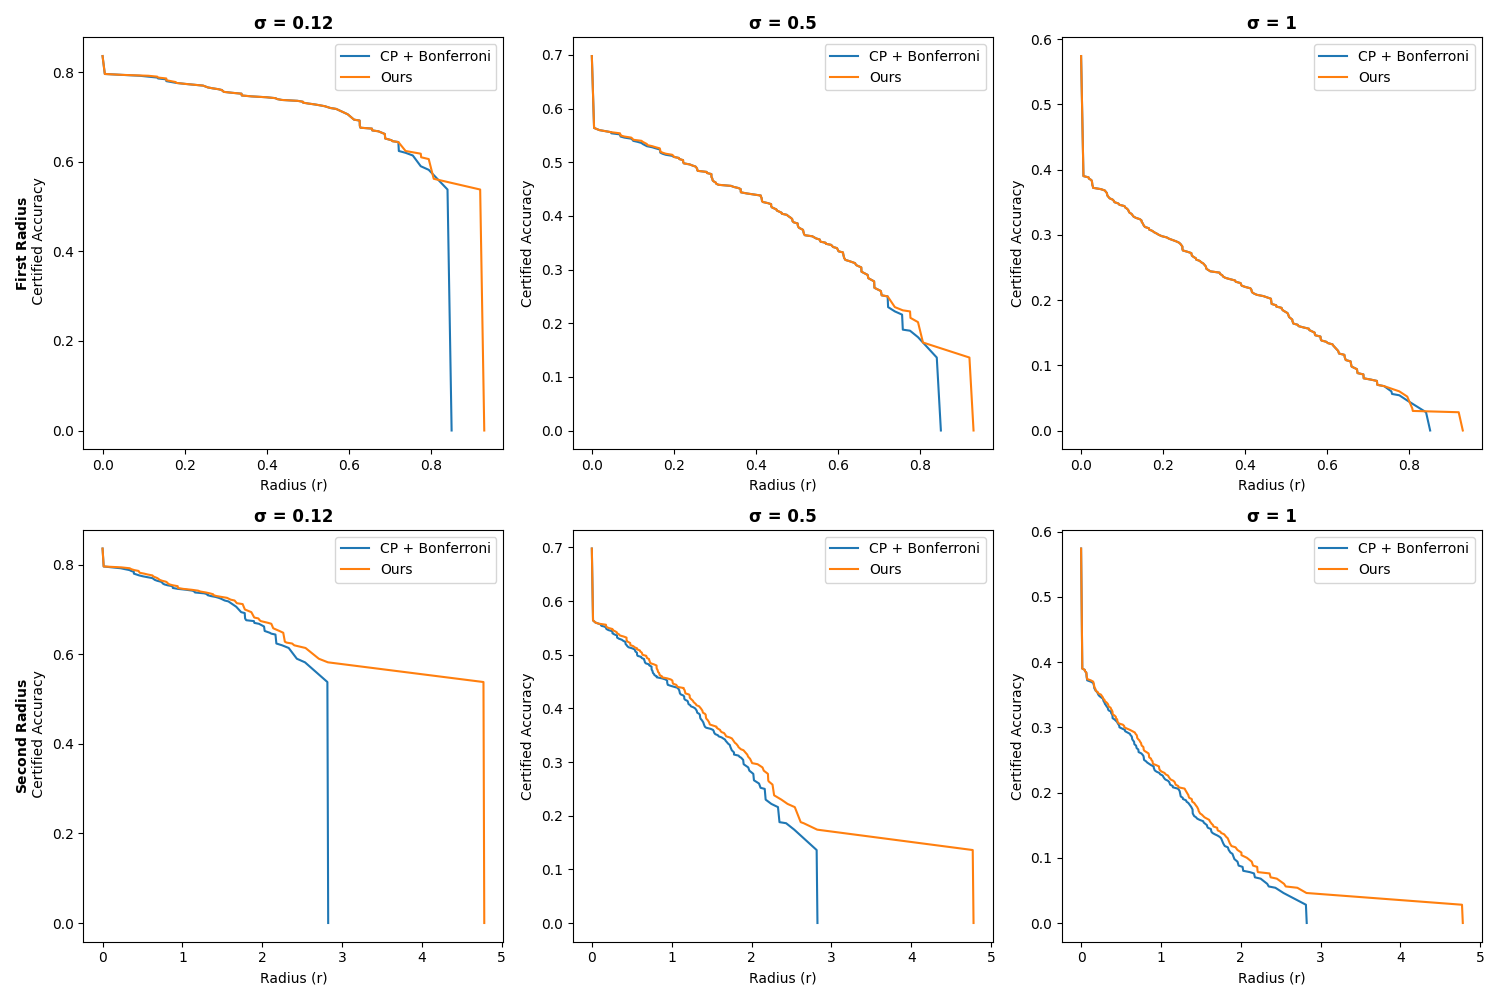
\includegraphics[width=0.8\textwidth]{images/discrete_sigma}
    \caption{Certified accuracies' comparison on the CIFAR-10 dataset in the discrete case for different standard deviations (displayed on the columns) with a sample size of $100$. The legend and row conventions are the same as in Figure~\ref{fig:discrete_num}.}
    \label{fig:discrete_sigma}
\end{figure}

In the continuous case, in addition to the sample size and the standard deviation, another hyperparameter to consider is the \textit{temperature}.
The simplex map $s$ used in the experiments is the tempered softmax function which is a generalization of the standard softmax function, introducing a temperature parameter to control the smoothness of the output distribution.
Given a vector $\mathbf{x} = (x_1, \ldots, x_m)$ and a temperature parameter $T > 0$, the tempered softmax function $\sigma_T: \mathbb{R}^m \to \mathbb{R}^m$ is defined as:
\[
    \sigma_T(\mathbf{x})_i = \frac{\exp(x_i/T)}{\sum_{j=1}^n \exp(x_j/T)}
\]
for $i = 1, \ldots, m$.

As $T \to 0^+$, the tempered softmax approaches a hard maximum (one-hot vector).
As $T \to \infty$, the tempered softmax approaches a uniform distribution.
When $T = 1$, it reduces to the standard softmax function.

Figures~\ref{fig:cont_num} \&~\ref{fig:cont_sigma} and tables~\ref{tab:certified-accuracy} \&~\ref{tab:certified-accuracy-2} show the effect of increasing the number of samples $n$ and increasing the standard deviation $\sigma$ respectively.
The effects of these hyperparameters are similar in both discrete and continuous case.
\begin{figure}[htbp]
    \centering
    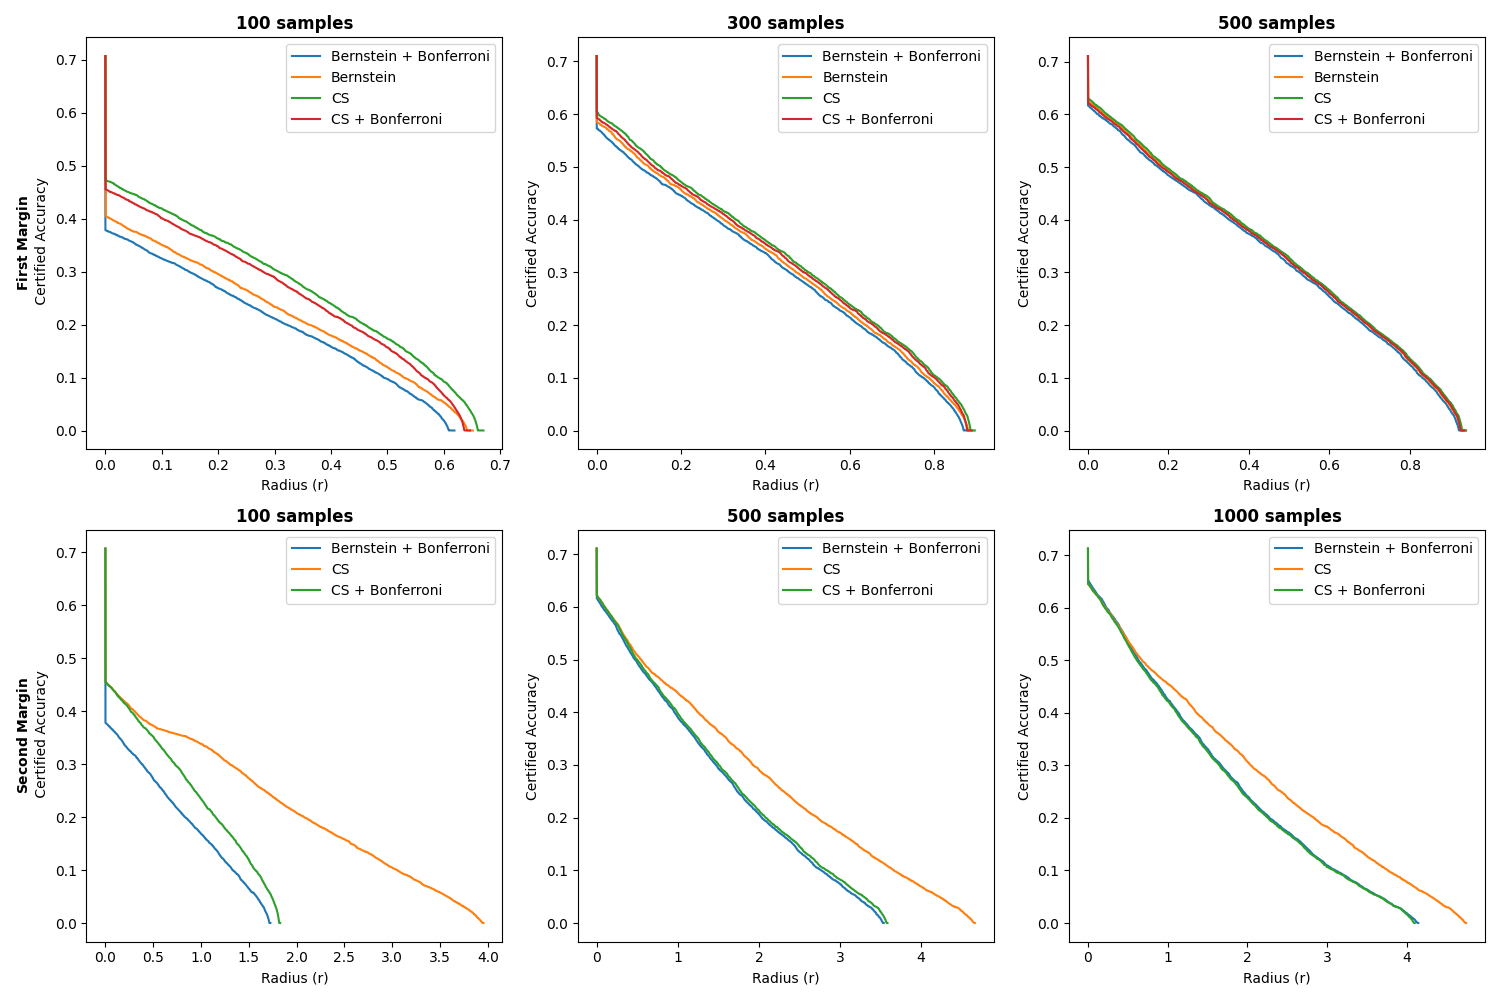
\includegraphics[width=0.8\textwidth]{images/cont_num}
    \caption{Certified accuracies' comparison on the CIFAR-10 dataset in the continuous case for different sample sizes (displayed on the columns) with $\sigma = 0.5$ and a temperature equal to $1$. CS/Bernstein + Bonferroni stands for the Bonferroni approach with either the empirical Bernstein interval (Proposition~\ref{prop:empirical-bernstein-inequality}) or the confidence sequence (Proposition~\ref{prop:confidence-sequence}), and CS/Bernstein + Ours stands for the new approach in section~\ref{sec:continuous}, where the interval used is either the empirical Bernstein interval or the confidence sequence as before. The first row compares the certified accuracies using the first margin and the second row compares the certified accuracies using the second margin.}
    \label{fig:cont_num}
\end{figure}
\begin{figure}[htbp]
    \centering
    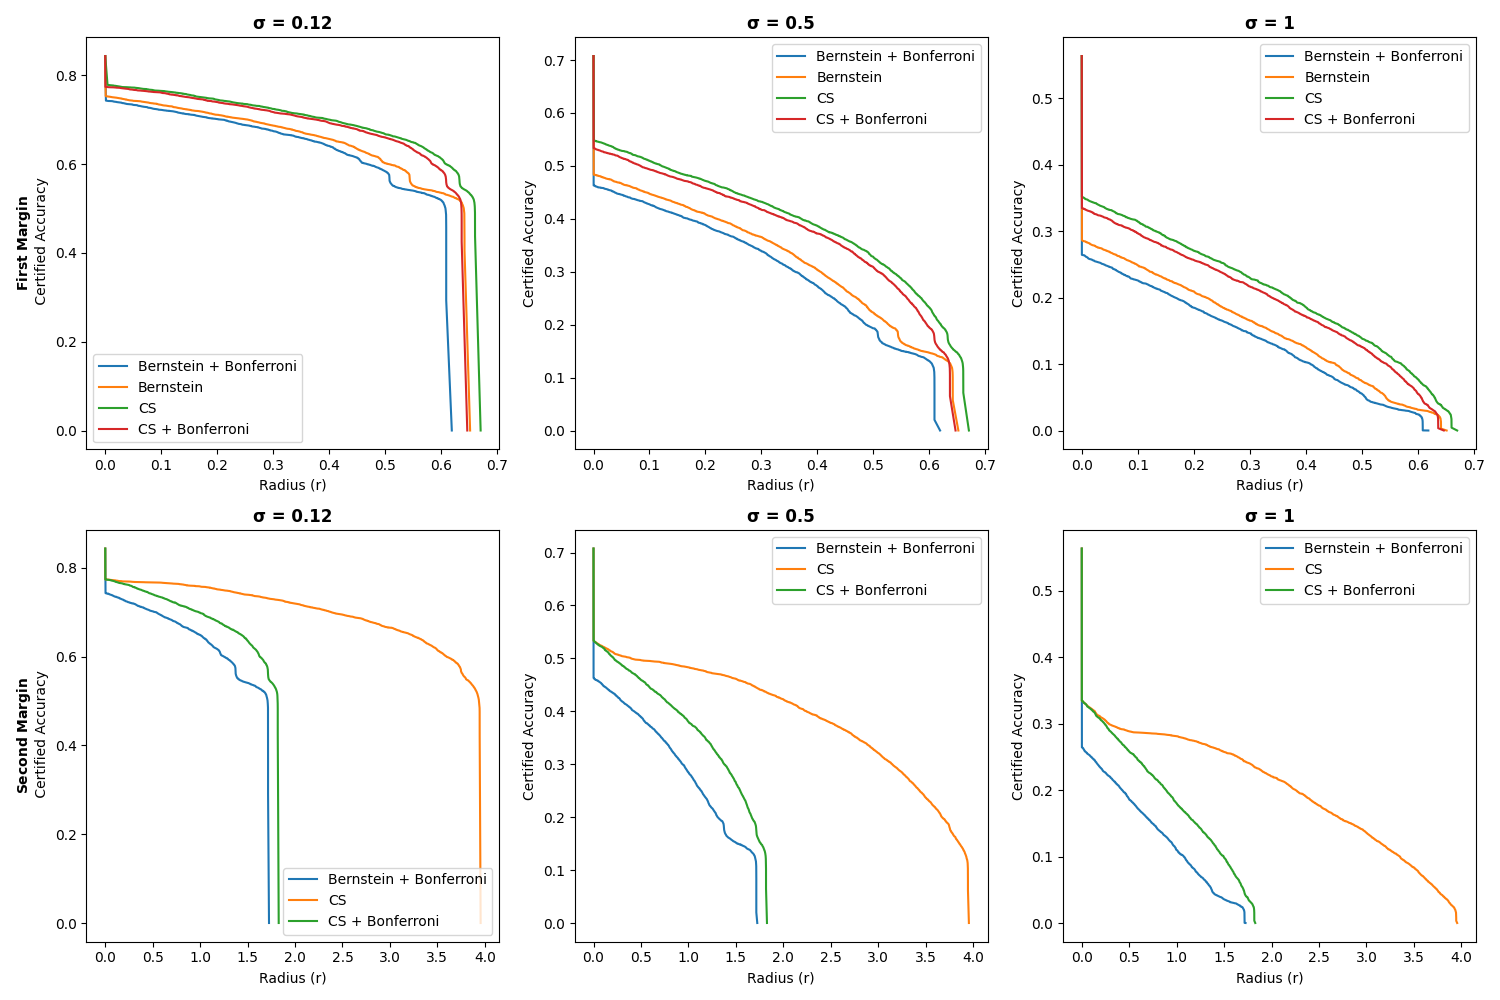
\includegraphics[width=0.8\textwidth]{images/cont_sigma}
    \caption{Certified accuracies' comparison on the CIFAR-10 dataset in the continuous case for different standard deviations (displayed on the columns) with a sample size of $100$ and a temperature equal to $0.1$. The legend and row conventions are the same as in Figure~\ref{fig:cont_num}.}
    \label{fig:cont_sigma}
\end{figure}
\begin{figure}[htbp]
    \centering
    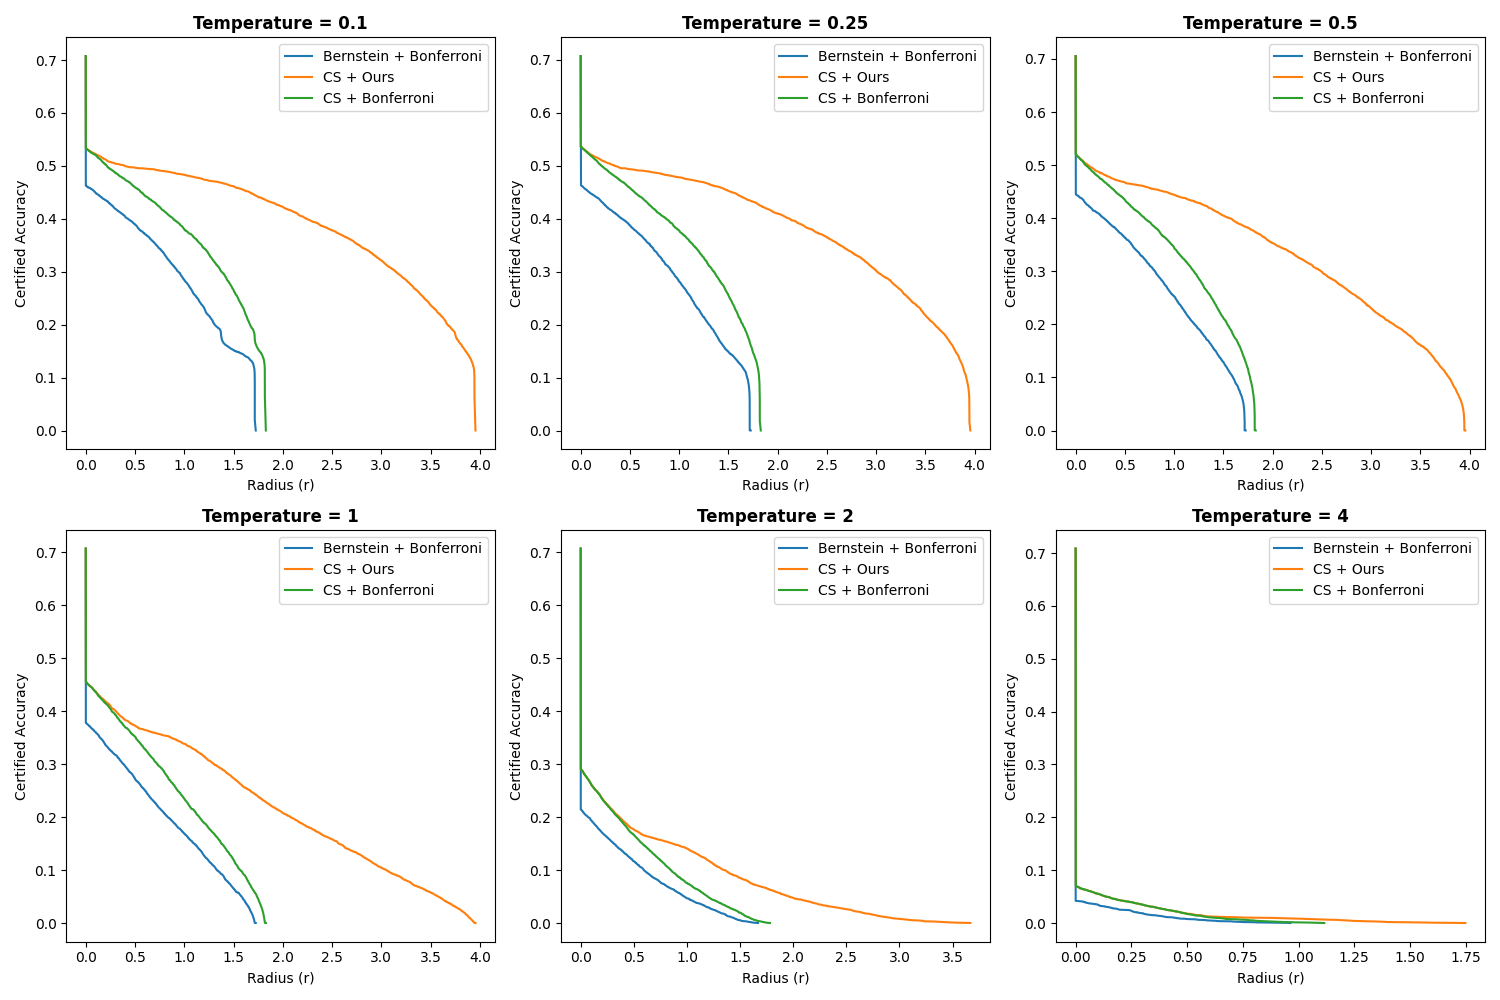
\includegraphics[width=0.8\textwidth]{images/cont_temp}
    \caption{Certified accuracies' comparison on the CIFAR-10 dataset in the continuous case for different temperatures (displayed on the columns) with a sample size of $100$ and $\sigma = 0.5$. The legend and row conventions are the same as in Figure~\ref{fig:cont_num}.}
    \label{fig:cont_temp}
\end{figure}

\begin{table}[htbp]
    \centering
    \caption{Certified accuracy using the first margin on CIFAR-10 in the continuous case for different values of radius $r$ and sample sizes with $\sigma = 0.5$ and a temperature of $1$.}
    \label{tab:certified-accuracy}
    \renewcommand{\arraystretch}{1.2}
    \begin{tabular}{@{}ll*{9}{c}@{}}
        \toprule
        \multirow{2}{*}{Samples} & \multirow{2}{*}{Method} & \multicolumn{9}{c}{Radius ($r$)} \\
        \cmidrule(l){3-11}
        & & 0.1 & 0.2 & 0.3 & 0.4 & 0.5 & 0.6 & 0.7 & 0.8 & 0.9 \\
        \midrule
        \multirow{3}{*}{100}
        & CS + Bonferroni & 0.400 & 0.347 & 0.289 & 0.220 & 0.157 & 0.066 & 0.000 & 0.000 & 0.000 \\
        & CS + Ours            & 0.419 & 0.362 & 0.303 & 0.239 & 0.173 & 0.092 & 0.000 & 0.000 & 0.000 \\
        & Comparison (\%) & 4.69\% & 4.28\% & 5.04\% & 8.70\% & 10.65\% & 39.16\% & N/A & N/A & N/A \\
        \midrule
        \multirow{3}{*}{300}
        & CS + Bonferroni & 0.526 & 0.464 & 0.411 & 0.354 & 0.296 & 0.233 & 0.173 & 0.101 & 0.000 \\
        & CS + Ours             & 0.536 & 0.471 & 0.416 & 0.361 & 0.301 & 0.239 & 0.179 & 0.105 & 0.000 \\
        & Comparison (\%) & 1.93\% & 1.55\% & 1.39\% & 1.89\% & 1.94\% & 2.52\% & 3.49\% & 4.06\% & N/A \\
        \midrule
        \multirow{3}{*}{500}
        & CS + Bonferroni & 0.560 & 0.490 & 0.434 & 0.379 & 0.322 & 0.261 & 0.199 & 0.133 & 0.050 \\
        & CS + Ours             & 0.568 & 0.497 & 0.442 & 0.383 & 0.329 & 0.266 & 0.202 & 0.136 & 0.054 \\
        & Comparison (\%) & 1.43\% & 1.33\% & 2.00\% & 0.99\% & 2.08\% & 2.01\% & 1.89\% & 2.33\% & 9.21\% \\
        \bottomrule
    \end{tabular}
\end{table}
\begin{table}[htbp]
    \centering
    \caption{Certified accuracy using the second margin on CIFAR-10 in the continuous case for different values of radius $r$ and sample sizes with $\sigma = 0.5$ and a temperature of $1$.}
    \label{tab:certified-accuracy-2}
    \renewcommand{\arraystretch}{1.2}
    \begin{tabular}{@{}ll*{9}{c}@{}}
        \toprule
        \multirow{2}{*}{Samples} & \multirow{2}{*}{Method} & \multicolumn{9}{c}{Radius ($r$)} \\
        \cmidrule(l){3-11}
        & & 0.1 & 0.2 & 0.3 & 0.4 & 0.5 & 0.6 & 0.7 & 0.8 & 0.9 \\
        \midrule
        \multirow{3}{*}{100}
        & CS + Bonferroni & 0.436 & 0.415 & 0.393 & 0.369 & 0.352 & 0.328 & 0.305 & 0.284 & 0.259 \\
        & CS + Ours             & 0.437 & 0.418 & 0.401 & 0.383 & 0.373 & 0.364 & 0.359 & 0.354 & 0.347 \\
        & Comparison (\%) & 0.19\% & 0.83\% & 1.91\% & 3.72\% & 5.95\% & 11.17\% & 17.68\% & 24.67\% & 34.03\% \\
        \midrule
        \multirow{3}{*}{300}
        & CS + Bonferroni & 0.572 & 0.545 & 0.518 & 0.493 & 0.471 & 0.451 & 0.431 & 0.413 & 0.391 \\
        & CS + Ours             & 0.572 & 0.547 & 0.523 & 0.500 & 0.481 & 0.465 & 0.451 & 0.439 & 0.427 \\
        & Comparison (\%) & 0.00\% & 0.42\% & 0.92\% & 1.46\% & 2.15\% & 2.97\% & 4.59\% & 6.25\% & 9.24\% \\
        \midrule
        \multirow{3}{*}{500}
        & CS + Bonferroni & 0.600 & 0.578 & 0.553 & 0.525 & 0.500 & 0.478 & 0.457 & 0.437 & 0.419 \\
        & CS + Ours             & 0.600 & 0.578 & 0.556 & 0.530 & 0.509 & 0.489 & 0.473 & 0.461 & 0.448 \\
        & Comparison (\%) & 0.08\% & 0.08\% & 0.53\% & 1.03\% & 1.77\% & 2.29\% & 3.50\% & 5.62\% & 6.98\% \\
        \bottomrule
    \end{tabular}
\end{table}

It is clear from Figure~\ref{fig:cont_temp} that increasing the temperature parameter $T$ reduces the discrepancies between the Bonferroni approach and our new method.
Higher temperatures lead to softer decision boundaries.
As the temperature increases, the output probabilities of the tempered softmax function become more uniform, regardless of the input values.
This means that the function becomes less sensitive to differences in the input, causing different methods to produce more similar outputs.
Hence, as the temperature rises, the tempered softmax function becomes less responsive to changes in its inputs.
This means that larger changes in the input are required to produce the same change in output probabilities.
Consequently, the differences between various methods become less pronounced.
At lower temperatures, the tempered softmax accentuates differences between inputs.
The highest value tends to dominate, resulting in an output distribution that's closer to a one-hot vector.
